\documentclass[tikz,border=8pt]{standalone}
% Shared look for every TikZ diagram. Load with % Shared look for every TikZ diagram. Load with % Shared look for every TikZ diagram. Load with \input{../../tools/tikz-style.tex}
\usepackage[T1]{fontenc}
\usepackage{lmodern}
\renewcommand{\sfdefault}{lmr}  % diagrams use the same serif as the text
\usetikzlibrary{arrows.meta, positioning, shapes.geometric, calc, fit, backgrounds}
\definecolor{cblue}{HTML}{4C78A8}
\definecolor{corange}{HTML}{F58518}
\definecolor{cgreen}{HTML}{54A24B}
\definecolor{cred}{HTML}{E45756}
\definecolor{cpurple}{HTML}{B279A2}
\definecolor{cgrey}{HTML}{6B6B6B}
\tikzset{
  every picture/.style={font=\sffamily, line width=1.2pt},
  box/.style={draw=#1, fill=#1!12, rounded corners=4pt, align=center, inner sep=7pt, minimum height=1.1cm},
  box/.default=cgrey,
  arrow/.style={-{Stealth[length=3mm]}, draw=cgrey, line width=1.4pt},
  title/.style={font=\sffamily\bfseries\Large},
  note/.style={font=\sffamily\small, text=cgrey, align=center},
}
\AtBeginDocument{\hyphenpenalty=10000 \exhyphenpenalty=10000}

\usepackage[T1]{fontenc}
\usepackage{lmodern}
\renewcommand{\sfdefault}{lmr}  % diagrams use the same serif as the text
\usetikzlibrary{arrows.meta, positioning, shapes.geometric, calc, fit, backgrounds}
\definecolor{cblue}{HTML}{4C78A8}
\definecolor{corange}{HTML}{F58518}
\definecolor{cgreen}{HTML}{54A24B}
\definecolor{cred}{HTML}{E45756}
\definecolor{cpurple}{HTML}{B279A2}
\definecolor{cgrey}{HTML}{6B6B6B}
\tikzset{
  every picture/.style={font=\sffamily, line width=1.2pt},
  box/.style={draw=#1, fill=#1!12, rounded corners=4pt, align=center, inner sep=7pt, minimum height=1.1cm},
  box/.default=cgrey,
  arrow/.style={-{Stealth[length=3mm]}, draw=cgrey, line width=1.4pt},
  title/.style={font=\sffamily\bfseries\Large},
  note/.style={font=\sffamily\small, text=cgrey, align=center},
}
\AtBeginDocument{\hyphenpenalty=10000 \exhyphenpenalty=10000}

\usepackage[T1]{fontenc}
\usepackage{lmodern}
\renewcommand{\sfdefault}{lmr}  % diagrams use the same serif as the text
\usetikzlibrary{arrows.meta, positioning, shapes.geometric, calc, fit, backgrounds}
\definecolor{cblue}{HTML}{4C78A8}
\definecolor{corange}{HTML}{F58518}
\definecolor{cgreen}{HTML}{54A24B}
\definecolor{cred}{HTML}{E45756}
\definecolor{cpurple}{HTML}{B279A2}
\definecolor{cgrey}{HTML}{6B6B6B}
\tikzset{
  every picture/.style={font=\sffamily, line width=1.2pt},
  box/.style={draw=#1, fill=#1!12, rounded corners=4pt, align=center, inner sep=7pt, minimum height=1.1cm},
  box/.default=cgrey,
  arrow/.style={-{Stealth[length=3mm]}, draw=cgrey, line width=1.4pt},
  title/.style={font=\sffamily\bfseries\Large},
  note/.style={font=\sffamily\small, text=cgrey, align=center},
}
\AtBeginDocument{\hyphenpenalty=10000 \exhyphenpenalty=10000}

\begin{document}
\begin{tikzpicture}[
  g/.style={circle, fill=cgreen, draw=black, line width=0.6pt, inner sep=3.2pt},
  r/.style={circle, fill=cred, draw=black, line width=0.6pt, inner sep=3.2pt},
  ring/.style={circle, draw=black, line width=1.4pt, minimum size=0.75cm}]
  \begin{scope}[rotate=20]
    \draw[line width=2.2pt] (-1,0) -- (8.5,0) node[right] {$w^{T}x + b = 0$ \quad ($\pi$)};
    \draw[dashed, cgrey, line width=1.4pt] (-1,1.4) -- (8.5,1.4) node[right, text=cgreen] {$w^{T}x + b = +1$ \quad ($\pi^{+}$)};
    \draw[dashed, cgrey, line width=1.4pt] (-1,-1.4) -- (8.5,-1.4) node[right, text=cred] {$w^{T}x + b = -1$ \quad ($\pi^{-}$)};
    \draw[{Stealth[length=3mm]}-{Stealth[length=3mm]}, line width=1.4pt] (0.4,-1.4) -- (0.4,1.4);
    \node[fill=white, inner sep=2pt, anchor=west] at (0.55,0.75) {$d = \dfrac{2}{\lVert w \rVert}$};
    \draw[-{Stealth[length=3.5mm]}, line width=2pt, cblue] (5.2,0) -- (5.2,1.1) node[above right=-2pt] {$w$};
    \node[g] (s1) at (3,1.4) {}; \node[ring] at (s1) {};
    \node[r] (s2) at (2.2,-1.4) {}; \node[ring] at (s2) {};
    \foreach \p in {(1,2.6),(4.5,2.5),(6.2,3.2),(7.5,2.1),(2.5,3.6)} \node[g] at \p {};
    \foreach \p in {(0.8,-2.5),(3.6,-2.4),(4.6,-3.4),(7.2,-2.4),(6,-1.9)} \node[r] at \p {};
  \end{scope}
  \node[font=\sffamily, text=cgreen, align=left] at (0.2,5.0) {green points: $y_i = +1$,\\ $w^{T}x_i + b \geq 1$};
  \node[font=\sffamily, text=cred, align=left] at (8.6,-1.2) {red points: $y_i = -1$,\\ $w^{T}x_i + b \leq -1$};
\end{tikzpicture}
\end{document}
